\documentclass{beamer}
\usepackage{beamerthemesplit}
\usepackage{wrapfig}
\usetheme{SPbGU}
\usepackage{pdfpages}
\usepackage{amsmath}
\usepackage{mathtools}
\usepackage{cmap}
\usepackage[T2A]{fontenc}
\usepackage[utf8]{inputenc}
\usepackage[english,russian]{babel}
\usepackage{indentfirst}
\usepackage{amsmath}
\usepackage{tikz}
\usepackage{multirow}
\usepackage[noend]{algpseudocode}
\usepackage{algorithm}
\usepackage{algorithmicx}
\usepackage{ stmaryrd }
\usepackage{fancyvrb}
\usepackage{qtree}
\usepackage{verbatim}
\newtheorem{rutheorem}{Теорема}
\newtheorem{ruproof}{Доказательство}
\newtheorem{rudefinition}{Определение}
\newtheorem{rulemma}{Лемма}
\beamertemplatenavigationsymbolsempty

\setbeamertemplate{itemize item}[circle]
\setbeamertemplate{enumerate item}[circle]
\newcommand{\derives}[1][*]{\xRightarrow[]{#1}}

\def\To{\derives[]}
\def\iff{\Leftrightarrow}

\usetikzlibrary{shapes,arrows}
\usetikzlibrary{positioning,automata}
\tikzset{every state/.style={minimum size=0.2cm},
initial text={}
}


\title[]{Теория автоматов и формальных языков}
\subtitle[]{Конечные автоматы}
\institute[]{
Санкт-Петербургский государственный электротехнический университет <<ЛЭТИ>>\\
}

\author[]{Екатерина Вербицкая}

\date{25 сентября 2020}

\definecolor{orange}{RGB}{179,36,31}

\begin{document}
{
  \begin{frame}
    \titlepage
  \end{frame}
}

\begin{frame}[fragile]
  \transwipe[direction=90]
  \frametitle{В предыдущей серии}
  \begin{itemize}
    \item Формальные языки повсюду. Язык --- множество строк над алфавитом
    \item Существует множество способов описать язык
    \item Задачи теории формальных языков
    \begin{itemize}
      \item Как представить язык?
      \item Какие есть характеристики у разных представлений языка?
      \item Как определить, принадлежит ли строка данному языку?
    \end{itemize}
  \end{itemize}
\end{frame}

\begin{frame}[fragile]
  \transwipe[direction=90]
  \frametitle{В предыдущей серии}
  \begin{itemize}
    \item Формальная грамматика
    \begin{itemize}
      \item $\langle$Терминалы, Нетерминалы, Правила, Стартовый нетерминал$\rangle$
    \end{itemize}
   \item Вывод: транзитивное и рефлексивное замыкание отношения выводимости
   \begin{itemize}
     \item Левосторонний (на каждом шаге заменяем самый левый нетерминал) и правосторонний
   \end{itemize}
   \item Дерево вывода
   \begin{itemize}
     \item Дерево: листья соответствуют терминалам, внутренние вершины --- нетерминалам; для каждого внутреннего узла существует правило грамматики, правая часть которого совпадает с метками детей узла
   \end{itemize}
    \item  Контекстно-свободная грамматика
      \begin{itemize}
        \item все правила имеют вид $A \rightarrow \alpha$

      \end{itemize}

      \end{itemize}

\end{frame}

\begin{frame}[fragile]
  \transwipe[direction=90]
  \frametitle{В предыдущей серии: левосторонний и правосторонний вывод}

\[
  \begin{array}{rcl}
  E& \rightarrow & E + E \mid N \\
  N& \rightarrow & 0 \mid 1  \\
  \end{array}
\]


\begin{center}
    Какой из нетерминалов раскрывать на данном шаге?
\end{center}

  \begin{itemize}
    \item Левосторонний вывод: раскрываем самый левый нетерминал
    \begin{itemize}
      \item $\boldsymbol{E} \To \boldsymbol{E} + E \To \boldsymbol{N} + E \To 1 + \boldsymbol{E} \To 1 + \boldsymbol{E} + E \derives[2] 1 + 0 + \boldsymbol{E} \derives[2] 1 + 0 + 1 $ \pause
	\end{itemize}
    \item Правосторонний вывод: раскрываем самый правый нетерминал
    \begin{itemize}
      \item $\boldsymbol{E} \To E + \boldsymbol{E} \To E + \boldsymbol{N} \To \boldsymbol{E} + 1 \To E + \boldsymbol{E} + 1 \derives[2] \boldsymbol{E} + 0 + 1 \derives[2] 1 + 0 + 1 $
	\end{itemize}
	\pause
	\item Для каких грамматик левосторонний и правосторонний вывод любой строки совпадают?
  \end{itemize}
\end{frame}

\begin{frame}[fragile]
  \transwipe[direction=90]
  \frametitle{Пример}
  Построить 2 различных (левосторонних) вывода строки $1+0+1$

\[
  \begin{array}{rcl}
  E& \rightarrow & E + E \mid N \\
  N& \rightarrow & 0 \mid 1  \\
  \end{array}
\]

    \begin{itemize}
      \item $\boldsymbol{E} \To \boldsymbol{E} + E \To \boldsymbol{N} + E \To 1 + \boldsymbol{E} \To 1 + \boldsymbol{E} + E \derives[2] 1 + 0 + \boldsymbol{E} \derives[2] 1 + 0 + 1 $ \pause
      \item $\boldsymbol{E} \To \boldsymbol{E} + E \To \boldsymbol{E} + E + E \To \boldsymbol{N} + E + E \To 1 + \boldsymbol{E} + E \derives[2] 1 + 0 + \boldsymbol{E} \derives[2] 1 + 0 + 1 $
	\end{itemize}
	\pause

\begin{tabular}{p{5.5cm} p{6cm}}

\Tree [.E [.E [.N 1 ] ] + [.E [.E [.N 0 ] ] + [.E [.N 1 ] ] ] ]
&
\Tree [.E [.E [.E [.N 1 ] ]  + [.E [.N 0 ] ] ] + [.E [.N 1 ] ] ]
\end{tabular}
\end{frame}

\begin{frame}[fragile]
  \transwipe[direction=90]
  \frametitle{Теоретико-множественное доказательство невозможности описания языков}

  \begin{center}
    Правда ли, что любой бесконечный язык можно представить конечным описанием?

    \pause \textbf{Нет.}
  \end{center}

  \begin{itemize}
    \item Конечное описание --- предложение над некоторым алфавитом (подразумеваемая интерпретация которого связывает его с описываемым языком) \pause
    \item Любой язык является не более, чем счетным; соответственно существует не более, чем счетное множество конечных описаний \pause
    \item Множество всех языков над данным алфавитом не является счетным, так как множество всех подмножеств счетного множества более, чем счетно \pause
    \item Итого, конечных описаний меньше, чем языков; соответственно не для всех бесконечных языков существует конечное описание
  \end{itemize}
\end{frame}

\begin{frame}[fragile]
  \transwipe[direction=90]
  \frametitle{Конечные автоматы}
  \begin{center}
    \begin{tikzpicture}[node distance=5cm, on grid]
      \node[state] (q_l)                {Locked};
      \node[state] (q_u) [right=of q_l] {Unlocked};
      \path[->] (q_l) edge [loop left]  node         {Push} ()
                      edge [bend left]  node [above] {Coin} (q_u)
                (q_u) edge [loop right] node         {Coin} ()
                      edge [bend left]  node [below] {Push} (q_l);
    \end{tikzpicture}
  \end{center}
\end{frame}

\begin{frame}[fragile]
  \transwipe[direction=90]
  \frametitle{Конечные автоматы}
  \begin{center}
     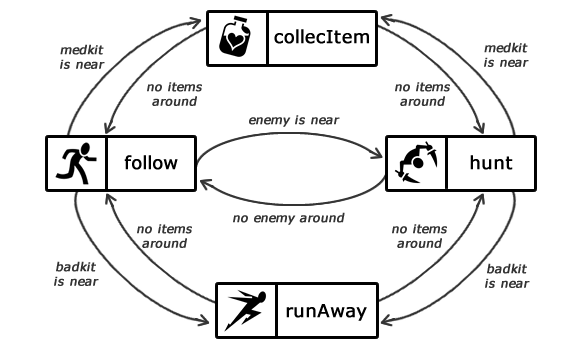
\includegraphics[width=0.85\textwidth]{pics/game.png}
   \end{center}
\end{frame}

\begin{frame}[fragile]
  \transwipe[direction=90]
  \frametitle{Конечные автоматы}
  \begin{center}
     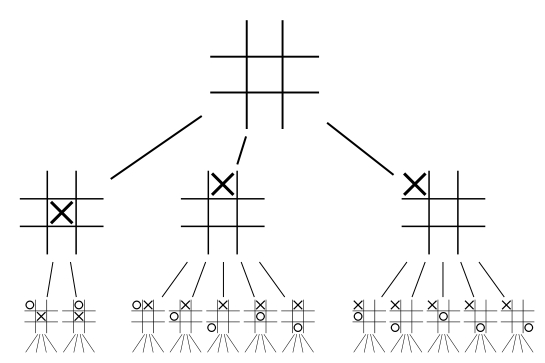
\includegraphics[width=0.85\textwidth]{pics/tictac.jpg}
   \end{center}
\end{frame}

\begin{frame}[fragile]
  \transwipe[direction=90]
  \frametitle{Конечный автомат}
  \textbf{(Детерминированный) конечный автомат} --- $\langle Q, \Sigma, \delta, q_0, F \rangle$
  \begin{itemize}
    \item $Q \neq \varnothing$ --- конечное множество состояний
    \item $\Sigma$ --- Конечный входной алфавит
    \item $\delta$ --- отображение типа $Q \times \Sigma \rightarrow Q$
    \begin{itemize}
      \item $\delta(q_i, x) = q_j$
    \end{itemize}
    \item $q_0 \in Q$ --- начальное состояние
    \item $F \subseteq Q$ --- множество конечных состояний
  \end{itemize}

  КА называется \textbf{полным}, если существует переход из каждого состояния по каждому символу алфавита
\begin{itemize}
    \item Обычно добавляют ``дьявольскую'' вершину, она же сток.
\end{itemize}
\end{frame}


\begin{frame}[fragile]
  \transwipe[direction=90]
  \frametitle{Пример конечного автомата}

\[
  Q = \{ q_0, q_1, q_2, q_3\}, \Sigma = \{ 0, 1, -\}, q_0 = q_0, F = \{q_1, q_2\}
\]

\begin{columns}
  \begin{column}{0.4\textwidth}
\[
\begin{array}{rcl}
  \delta (q_0, 0) &=& q_1 \\
  \delta (q_0, 1) &=& q_2 \\
  \delta (q_0, -) &=& q_3 \\
  \delta (q_2, 0) &=& q_2 \\
  \delta (q_2, 1) &=& q_2 \\
  \delta (q_3, 1) &=& q_2
\end{array}
\]
  \end{column}

  \begin{column}{0.6\textwidth}
    \begin{center}
      \begin{tikzpicture}[node distance=2cm, on grid]
        \node[state]           (q_3)                      {$q_3$};
        \node[state,initial]   (q_0) [above left=of q_3]  {$q_0$};
        \node[state,accepting] (q_1) [below left=of q_3]  {$q_1$};
        \node[state,accepting] (q_2) [above right=of q_3] {$q_2$};

        \path[->] (q_0) edge [bend left]  node [above] {$1$}       (q_2)
                        edge              node [left]  {$0$}       (q_1)
                        edge              node [above] {$-$}       (q_3)
                  (q_3) edge              node [above] {$1$}       (q_2)
                  (q_2) edge [loop above] node         {$0$}       ()
                        edge [loop below] node         {$1$}       ();
      \end{tikzpicture}
    \end{center}
  \end{column}
\end{columns}


\end{frame}

\begin{frame}[fragile]
  \transwipe[direction=90]
  \frametitle{Пример полного конечного автомата}
  \begin{center}
    \begin{tikzpicture}[node distance=2cm, on grid]
      \node[state]           (q_3)                      {$q_3$};
      \node[state,initial]   (q_0) [above left=of q_3]  {$q_0$};
      \node[state,accepting] (q_1) [below left=of q_3]  {$q_1$};
      \node[state,accepting] (q_2) [above right=of q_3] {$q_2$};
      \node[state]           (q_d) [below right=of q_3] {$D$};

      \path[->] (q_0) edge [bend left]  node [above] {$1$}       (q_2)
                      edge              node [left]  {$0$}       (q_1)
                      edge              node [above] {$-$}       (q_3)
                (q_3) edge              node [above] {$1$}       (q_2)
                      edge              node [above] {$\ \ 0, -$}(q_d)
                (q_2) edge [loop above] node         {$0$}       ()
                      edge [loop below] node         {$1$}       ()
                      edge [bend left]  node [right] {$-$}       (q_d)
                (q_1) edge              node [above] {$0, 1, -$} (q_d)
                (q_d) edge [loop right] node         {$0, 1, -$} ();
    \end{tikzpicture}
  \end{center}
\end{frame}

\begin{frame}[fragile]
  \transwipe[direction=90]
  \frametitle{Путь в конечном автомате}
  \begin{itemize}
    \item \textbf{Путь} --- кортеж $\langle q_0, e_1, q_1, \dots, e_n, q_n\rangle$
    \begin{itemize}
      \item $n \geq 0$
      \item $\forall i: e_i = \langle q_{i-1}, w_i, q_i \rangle, \text{где } \delta(q_{i-1}, w_i) = q_i$
      \item $q_0$ --- \textbf{начало} пути
      \item $q_n$ --- \textbf{конец} пути
      \item $w_1, w_2, \dots, w_n$ --- \textbf{метка} пути
      \item $n$ --- \textbf{длина} пути
    \end{itemize}
    \item Путь \textbf{успешен}, если $q_0$ --- начальное состояние, а $q_n \in F$
    \item Состояние $q$ \textbf{достижимо} из состояния $p$, если существует путь из состояния $p$ в состояние $q$
  \end{itemize}
\end{frame}

\begin{frame}[fragile]
  \transwipe[direction=90]
  \frametitle{Пример пути}

  \begin{center}
    Успешный путь с меткой $\boldsymbol{-110}$ длины 4
  \end{center}

  \[
    \langle q_0, \langle q_0, -, q_3 \rangle, q_3, \langle q_3, 1, q_2 \rangle, q_2, \langle q_2, 1, q_2 \rangle, q_2, \langle q_2, 0, q_2 \rangle, q_2\rangle
  \]

  \begin{center}
    \begin{tikzpicture}[node distance=2cm, on grid]
      \node[state]           (q_3)                      {$q_3$};
      \node[state,initial]   (q_0) [above left=of q_3]  {$q_0$};
      \node[state,accepting] (q_1) [below left=of q_3]  {$q_1$};
      \node[state,accepting] (q_2) [above right=of q_3] {$q_2$};

      \path[->] (q_0) edge [bend left]  node [above] {$1$}       (q_2)
                      edge              node [left]  {$0$}       (q_1)
                      edge              node [above] {$-$}       (q_3)
                (q_3) edge              node [above] {$1$}       (q_2)
                (q_2) edge [loop above] node         {$0$}       ()
                      edge [loop below] node         {$1$}       ();
    \end{tikzpicture}
  \end{center}
\end{frame}

\begin{frame}[fragile]
  \transwipe[direction=90]
  \frametitle{Такт работы КА (шаг)}
  \begin{itemize}
    \item \textbf{Конфигурация (Мгновенное описание)} КА --- $\langle q, \omega \rangle$, где $q \in Q, \omega \in \Sigma^*$
    \item \textbf{Такт работы} --- бинарное отношение $\vdash$: если $\delta(p , x) = q$ и $\omega \in \Sigma ^*$, то $\langle p , x \omega \rangle \vdash \langle q , \omega \rangle$
    \item Бинарное отношение $\vdash^*$ --- рефлексивное, транзитивное замыкание $\vdash$
  \end{itemize}
\end{frame}

\begin{frame}[fragile]
  \transwipe[direction=90]
  \frametitle{Распознавание слова конечным автоматом}

\begin{center}
  Цепочка $\omega$ \textbf{распознается} КА, если $\exists$ успешный путь с меткой $\omega$
\end{center}

\vspace{20pt}

\begin{center}
  \textbf{Язык, распознаваемый конечным автоматом}: \\ $\{ \omega \in \Sigma^* \mid \exists p$ --- успешный путь с меткой $\omega \}$
\end{center}
\end{frame}

\begin{frame}[fragile]
  \transwipe[direction=90]
  \frametitle{Распознавание слова конечным автоматом: пример}

\[ \{ \dots, -110, -101, -100, -11, -10, -1, 0, 1, 10, 11, 100, 101, 110, \dots\} \]

\begin{center}
  Язык всех целых чисел в двоичной записи
\end{center}

  \begin{center}
    \begin{tikzpicture}[node distance=2cm, on grid]
      \node[state]           (q_3)                      {$q_3$};
      \node[state,initial]   (q_0) [above left=of q_3]  {$q_0$};
      \node[state,accepting] (q_1) [below left=of q_3]  {$q_1$};
      \node[state,accepting] (q_2) [above right=of q_3] {$q_2$};

      \path[->] (q_0) edge [bend left]  node [above] {$1$}       (q_2)
                      edge              node [left]  {$0$}       (q_1)
                      edge              node [above] {$-$}       (q_3)
                (q_3) edge              node [above] {$1$}       (q_2)
                (q_2) edge [loop above] node         {$0$}       ()
                      edge [loop below] node         {$1$}       ();
    \end{tikzpicture}
  \end{center}
\end{frame}


\begin{frame}[fragile]
  \transwipe[direction=90]
  \frametitle{Распознавание слова конечным автоматом}
  \begin{rutheorem}[]
   Рассмотрим конечный автомат  $M = \langle Q , \Sigma , \delta , q_0 , F \rangle$.

   Слово $\omega \in \Sigma ^*$ принадлежит языку $L(M) \iff \exists q \in F: \langle q_0 , \omega \rangle \vdash^* \langle q , \varepsilon \rangle$.
  \end{rutheorem}
\end{frame}

\begin{frame}[fragile]
  \transwipe[direction=90]
  \frametitle{Распознавание слова конечным автоматом}
   Обобщаем функцию перехода:

      \begin{itemize}
        \item $\delta' (q, \varepsilon) = q$
        \item $\delta' (q, x\alpha) = \delta'(\delta(q, x), \alpha) \text{, где } x \in \Sigma, \alpha \in \Sigma^*$
      \end{itemize}

  \begin{rutheorem}[]
     $\text{Цепочка } \omega \textbf{ распознается} \text{ КА } \langle Q, \Sigma, \delta, q_0, F \rangle \iff \exists p \in F : \delta'(q_0, \omega) = p$
  \end{rutheorem}


\begin{center}
     \textbf{Язык, распознаваемый конечным автоматом}: $\{ \omega \in \Sigma^* \mid \exists p \in F : \delta'(q_0, \omega) = p \}$
\end{center}
\end{frame}


\begin{frame}[fragile]
  \transwipe[direction=90]
  \frametitle{Свойство конкатенации строк}
  \begin{rutheorem}[]
    $\langle q_1 , \alpha \rangle \vdash^* \langle q_2 , \varepsilon \rangle, \langle q_2 , \beta \rangle \vdash^* \langle q_3 , \varepsilon \rangle \Rightarrow \langle q_1 , \alpha \beta \rangle \vdash^* \langle q_3 , \varepsilon \rangle$
  \end{rutheorem}
\end{frame}


\begin{frame}[fragile]
  \transwipe[direction=90]
  \frametitle{Эквивалентность конечных автоматов}
    \begin{center}
      Конечные автоматы $A_1$ и $A_2$ \textbf{эквивалентны}, если распознают один и тот же язык
    \end{center}

    \vspace{20pt}

    \begin{center}
      Как проверить что автоматы эквиваленты?
    \end{center}

\end{frame}

\begin{frame}[fragile]
  \transwipe[direction=90]
  \frametitle{Проверка на эквивалентность автоматов}
  \begin{itemize}
    \item Запустить одновременный обход в ширину двух автоматов
    \item Каждый переход должен приводить в терминальные или нетерминальные вершины в обоих автоматах соответственно
  \end{itemize}
\end{frame}

\begin{frame}[fragile]
  \transwipe[direction=90]
  \frametitle{Минимальный конечный автомат}
   \textbf{Минимальный конечный автомат} --- автомат, имеющий наименьшее число состояний, распознающий тот же язык, что и данный
\end{frame}

\begin{frame}[fragile]
  \transwipe[direction=90]
  \frametitle{Классы эквивалентности}
    \textbf{Отношение эквивалентности} --- рефлексивное, симметричное, транзитивное отношение
    \begin{itemize}
      \item $xRx$
      \item $xRy \iff yRx$
      \item $xRy, yRz \Rightarrow xRz$
    \end{itemize}

    \begin{rutheorem}
       $\forall R$ --- отношение эквивалентности на множестве $S$

      Можно разбить $S$ на $k$ непересекающихся подмножеств $I_1 \dots I_k$, т.ч. $aRb \iff a, b \in I_j$
    \end{rutheorem}


\begin{center}
      Множества $I_1 \dots I_k$ называются \textbf{классами эквивалентности}
\end{center}
\end{frame}

\begin{frame}[fragile]
  \transwipe[direction=90]
  \frametitle{Эквивалентные состояния}
  \begin{itemize}
    \item $\omega \in \Sigma^*$ \textbf{различает} состояния $q_i$ и $q_j$, если $\delta' (q_i, \omega) = t_1, \delta' (q_j, \omega) = t_2 \Rightarrow (t_1 \notin F \iff t_2 \in F)$
    \item $q_i$ и $q_j$ \textbf{эквивалентны} $(q_i \sim q_j)$, если $\forall \omega \in \Sigma^*: \delta' (q_i, \omega) = t_1, \delta' (q_j, \omega) = t_2 \Rightarrow (t_1 \in F \iff t_2 \in F)$
    \begin{itemize}
      \item Является отношением эквивалентности
    \end{itemize}
  \end{itemize}
   \begin{rulemma}
      $\mathcal{A} = \langle Q, \Sigma, \delta, q_0, F \rangle, p_1, p_2, q_1, q_2 \in Q, q_i = \delta(p_i, c)$

      $\omega \in \Sigma^*$ различает $q_1$ и $q_2$. Тогда $c \omega$ различает $p_1$ и $p_2$
   \end{rulemma}

   \begin{ruproof}
     $\delta' (p_i, c \omega) = \delta' (\delta (p_i, c), \omega) = \delta' (q_i, \omega) = t_i$
   \end{ruproof}
\end{frame}

\begin{frame}[fragile]
  \transwipe[direction=90]
  \frametitle{Алгоритм минимизации КА}
    TLDR: разбиваем состояния на классы эквивалентности, которые делаем новыми состояниями

\end{frame}

\begin{frame}[fragile]
  \transwipe[direction=90]
  \frametitle{Алгоритм минимизации КА}

     $Q$ --- очередь

     \vspace{10pt}

     $marked$ --- таблица размером $n \times n$ (n --- количество состояний КА).

     \vspace{10pt}

      Помечаем в таблице пары неэквивалентных состояний и кладем их в очередь

\end{frame}

\begin{frame}[fragile]
  \transwipe[direction=90]
  \frametitle{Алгоритм минимизации КА}
    \begin{itemize}
      \item Если автомат не полный --- дополнить дьявольской вершиной
      \item Строим отображение $\delta^{-1}$ --- обратные ребра
      \item Находим все достижимые из стартового состояния
      \item Добавляем в $Q$ и отмечаем в $marked$ пары состояний, различимые $\varepsilon$
      \item Можем пометить пару $(u, v)$, если $\exists c \in \Sigma :  (\delta(u, c), \delta(v, c)) помечена$. Для этого, пока $Q \neq \varnothing$:
      \begin{itemize}
        \item Извлекаем $(u, v)$ из $Q$
        \item $\forall c \in \Sigma$ перебираем $(\delta^{-1}(u, c), \delta^{-1}(v, c))$ --- если пара не помечена, помечаем и кладем в очередь
      \end{itemize}
      \item В момент опустошения $Q$ непомеченные пары являются эквивалентными
      \item За проход по таблице выделяем классы эквивалентности
      \item За проход по таблице формируем новые состояния и переходы
    \end{itemize}

\end{frame}

\begin{frame}[fragile]
  \transwipe[direction=90]
  \frametitle{Алгоритм минимизации КА}
    \begin{itemize}
      \item Стартовое состояние --- класс эквивалентности, которому принадлежит стартовое состояние исходного КА
      \item Конечные состояния --- классы эквивалентности, которым принадлежат конечные состояния исходного КА
    \end{itemize}

\end{frame}

\begin{frame}[fragile]
  \transwipe[direction=90]
  \frametitle{Алгоритм минимизации КА: корректность}
    \begin{itemize}
      \item Пусть в результате применения алгоритма к КА $A$ получили КА $A_{min}$. Покажем, что этот автомат минимальный и единственный с точностью до изоморфизма
      \item Пусть $\exists A' : A'$ и $A$ эквивалентны, но количество состояний $A'$ меньше, чем у $A_{min}$
      \item Стартовые состояния $s \in A_{min}$ и $s' \in A'$ эквивалентны (КА допускают один язык)
      \item $\sphericalangle \alpha = a_1 a_2 \dots a_k, a_i \in \Sigma: \langle s, \alpha \rangle \vdash^* \langle u, \varepsilon \rangle; \langle s', \alpha \rangle \vdash^* \langle u', \varepsilon \rangle$
      \item $\sphericalangle \langle s, a_1 \rangle \vdash^* \langle l, \varepsilon \rangle; \langle s', a_1 \rangle \vdash^* \langle l', \varepsilon \rangle$. $s, s'$ эквивалентны $\Rightarrow l, l'$ эквивалентны
      \item Аналогично для всех $a_i \Mapsto u, u'$ эквивалентны
      \item $\Mapsto \forall q$ --- состояние $A_{min} \exists q'$ --- эквивалентное состояние $A'$
      \item Состояний $A'$ меньше, чем состояний $A_{min} \Rightarrow$ 2 состояниям $A_{min}$ соответствует 1 состояние $A' \Rightarrow$ они эквивалентны. Но по построению $A_{min}$ в нем не может быть эквивалентных состояний. Противоречие
    \end{itemize}

\end{frame}

\begin{frame}[fragile]
  \transwipe[direction=90]
  \frametitle{Недетерминированный КА}
 \textbf{Недетерминированный конечный автомат} --- $\langle Q, \Sigma, \delta, q_0, F \rangle$
  \begin{itemize}
    \item $Q \neq \varnothing$ --- конечное множество состояний
    \item $\Sigma$ --- Конечный входной алфавит
    \item $\delta$ --- отображение типа $Q \times \Sigma \rightarrow 2^Q$
    \begin{itemize}
      \item $\delta(q_i, x) = \{ q_{j_0} \dots q_{j_k} \}$
    \end{itemize}
    \item $q_0 \in Q$ --- начальное состояние
    \item $F \subseteq Q$ --- множество конечных состояний
  \end{itemize}

\end{frame}

\begin{frame}[fragile]
  \transwipe[direction=90]
  \frametitle{Недетерминированный КА: пример}

\begin{columns}
  \begin{column}{0.25\textwidth}
\[
  \begin{array}{rcl}
    \delta (q_0, \text{а}) &=& q_0 \\
     &\dots&  \\
    \delta (q_0, \text{к}) &=& q_0 \\
    &\dots&  \\
    \delta (q_0, \text{я}) &=& q_0 \\

    \delta (q_0, \text{к}) &=& q_1 \\

    & & \\

    \delta (q_1, \text{о}) &=& q_2 \\

    & & \\

    \delta (q_2, \text{т}) &=& q_3 \\

    & & \\

    \delta (q_3, \text{а}) &=& q_3 \\
    &\dots&  \\
   \delta (q_3, \text{я}) &=& q_3 \\
  \end{array}
\]
  \end{column}

  \begin{column}{0.75\textwidth}
      \begin{center}
        \begin{tikzpicture}[node distance=2cm, on grid]
          \node[state,initial]   (q_0)                 {$q_0$};
          \node[state]           (q_1) [right =of q_0] {$q_1$};
          \node[state]           (q_2) [right =of q_1] {$q_2$};
          \node[state,accepting] (q_3) [right =of q_2] {$q_3$};

          \path[->] (q_0) edge node [above] {к} (q_1)
                          edge [loop above] node [above] {a\dots к\dots я} ()
                    (q_1) edge node [above] {о} (q_2)
                    (q_2) edge node [above] {т} (q_3)
                    (q_3) edge [loop above] node [above] {a\dots я} ();
        \end{tikzpicture}
      \end{center}
  \end{column}
\end{columns}
\end{frame}

\begin{frame}[fragile]
  \transwipe[direction=90]
  \frametitle{Распознавание слова НКА}
  \begin{itemize}
    \item \textbf{Конфигурация (Мгновенное описание)} КА --- $\langle q, \omega \rangle$, где $q \in Q, \omega \in \Sigma^*$
    \item \textbf{Такт работы} --- бинарное отношение $\vdash$: если $q \in \delta(p, x)$ и $\omega \in \Sigma ^*$, то $\langle p , x \omega \rangle \vdash \langle q , \omega \rangle$
    \item Бинарное отношение $\vdash^*$ --- рефлексивное, транзитивное замыкание $\vdash$
    \item НКА \textbf{допускает} слово $\alpha$, если $\exists t \in F : \langle s, \alpha \rangle \vdash^* \langle t, \varepsilon \rangle$
    \item \textbf{Язык НКА} $L(A) = \{ \omega \in \Sigma^* \mid \exists t \in F : \langle s, \omega \rangle \vdash^* \langle t, \varepsilon \rangle \}$
  \end{itemize}
  \begin{itemize}
    \item ДКА --- частный случай НКА
  \end{itemize}
\end{frame}

\begin{frame}[fragile]
  \transwipe[direction=90]
  \frametitle{Недетерминированный КА: пример}

      \begin{center}
        \begin{tikzpicture}[node distance=2cm, on grid]
          \node[state,initial]   (q_0)                 {$q_0$};
          \node[state]           (q_1) [right =of q_0] {$q_1$};
          \node[state]           (q_2) [right =of q_1] {$q_2$};
          \node[state,accepting] (q_3) [right =of q_2] {$q_3$};

          \path[->] (q_0) edge node [above] {к} (q_1)
                          edge [loop above] node [above] {a\dots к\dots я} ()
                    (q_1) edge node [above] {о} (q_2)
                    (q_2) edge node [above] {т} (q_3)
                    (q_3) edge [loop above] node [above] {a\dots я} ();
        \end{tikzpicture}
      \end{center}

\vspace{20pt}

  \begin{center}
    \{\textbf{кот}, с\textbf{кот}, \textbf{кот}лета, мя\textbf{кот}ь, антре\textbf{кот}\dots \}
  \end{center}
\end{frame}

\begin{frame}[fragile]
  \transwipe[direction=90]
  \frametitle{Алгоритм, определяющий допустимость слова}

\[
\begin{array}{rcl}
  R(\alpha)      &=& \{ p \mid \langle q_0, \alpha \rangle \vdash^* \langle p, \varepsilon \rangle\} \\
  & & \\
  R(\varepsilon) &=& \{q_0\} \\
  R(\alpha c)    &=& \{q \mid q \in \delta (p, c), p \in R(\alpha)\}
\end{array}
\]

\vspace{20pt}

\begin{center}
  НКА допускает слово $\alpha \iff \exists t \in F : t \in R(\alpha) $
\end{center}

\end{frame}

\begin{frame}[fragile]
  \transwipe[direction=90]
  \frametitle{Построение ДКА по НКА: алгоритм Томпсона}
  \begin{itemize}
    \item Помещаем в $Queue$ множество $\{ q_0 \}$
    \item Пока очередь не пуста, выполняем:
    \begin{itemize}
      \item $q = Queue.pop()$
      \item Строим множество $q' = \{t = \delta (s, c) \mid s \in q, c \in \Sigma\}$. Если $q' \notin Queue$, добавить его в очередь. Каждое такое множество --- новая вершина ДКА; добавляем переходы по соответствующим символам
      \item Если во множестве есть хотя бы одна вершина, являющаяся терминальной в данном НКА, то соответствующая вершина ДКА будет конечной
    \end{itemize}
  \item Результат: $\langle \Sigma, Q_d, q_{d_0} \in Q_d, F_d \subset Q_d, \delta_d: Q_d \times \Sigma \rightarrow {Q_d} \rangle$
  \begin{itemize}
    \item $Q_d = \{q_d \mid q_d \subset 2^Q \}$
    \item $q_{d_0} = \{q_0\}$
    \item $F_d = \{q \in Q_d \mid \exists p \in F : p \in q\}$
    \item $\delta_d(q, c) = \{ \delta(a, c) \mid a \in q \}$
  \end{itemize}
  \end{itemize}
\end{frame}

\begin{frame}[fragile]
  \transwipe[direction=90]
  \frametitle{Детерминизация НКА: пример}
    \begin{center}
      \begin{tikzpicture}[node distance=2cm, on grid]
        \node[state,initial]   (q_0)                 {$1$};
        \node[state,accepting] (q_1) [right =of q_0] {$2$};

        \path[->] (q_0) edge [bend left]  node [above] {a}   (q_1)
                        edge [loop above] node [above] {a,b} ()
                  (q_1) edge [bend left]  node [below] {b}   (q_0)
                        edge [loop above] node [above] {b}   ();
      \end{tikzpicture}
    \end{center}

    \begin{center}
      \begin{tikzpicture}[node distance=2cm, on grid]
        \node[state,initial]   (q_0)                 {$1$};
        \node[state,accepting] (q_1) [right =of q_0] {$1, 2$};

        \path[->] (q_0) edge              node [above] {a}   (q_1)
                        edge [loop above] node [above] {b}   ()
                  (q_1) edge [loop above] node [above] {a,b} ();
      \end{tikzpicture}
    \end{center}

\end{frame}



\begin{frame}[fragile]
  \transwipe[direction=90]
  \frametitle{Эквивалентность языков, распознаваемых ДКА и НКА}
  \begin{rutheorem}
  ДКА и НКА распознают один и тот же класс языков
  \end{rutheorem}
  \begin{proof}
  $\Rightarrow: $ очевидно

  $\Leftarrow: $ Рассмотрим произвольный НКА и покажем, что алгоритм Томпсона строит по нему эквивалентный ДКА.

  $\forall q \in q_d, \forall c \in \Sigma, \forall p \in \delta(q, c): p \in \delta_d (q_d, c)$

  Рассмотрим $\langle q_0, w_1 w_2 \dots w_m \rangle \vdash \langle u_1, w_2 \dots w_m\rangle  \vdash^* \langle u_m, \varepsilon \rangle, u_m \in F $

  $\forall i: u_i \in u_{d_i}, $ где $(q_{d_0}, w_1 w_2 \dots w_m) \vdash (u_{d_1}, w_2 \dots w_m) \vdash^* (u_{d_m}, \varepsilon)$

  $\Mapsto u_m \in u_{d_m}$
  \end{proof}
\end{frame}

\end{document}
